\documentclass[12pt, letterpaper]{article}
\usepackage{amsmath}
\usepackage{graphicx}
\graphicspath{{img/}}
\usepackage{amsmath}
\usepackage{amssymb}
\title{\huge\textbf{Moogle!}\thanks{\small Informe generado en \LaTeX}}
\author{\large Karla Díaz Saura\\ \small C113}
\date{\small Curso 2023}

\begin{document}
\maketitle

\newpage
\tableofcontents

\newpage
\section{Introducción}
La recuperación de la información es la organización, almacenamiento, recuperación y evaluación de la información de colecciones de documentos, en particular, la información textual. La recuperación de esta información es la actividad de obtener material (generalmente textos) que satisface una necesidad de información dentro de grandes colecciones almacenadas en computadoras. Los sistemas de recuperación permiten a los usuarios encontrar la información deseada, no explícitamente sino señalando la existencia y ubicación de documentos que pudieran contenerla.

Un sistema de recuperación de la información tiene la capacidad de representar, almacenar, organizar y acceder a elementos de información para satisfacer la necesidad de información en una larga colección de documentos. Se requiere un conjunto de palabras claves para buscar la información, estas resumen la descripción de la información deseada por el usuario. Las palabras claves son las consultas hechas por el usuario en los motores de búsqueda. 

\section{Moogle!}
    Mi versión de \textbf{Moogle!} consiste en un sistema de recuperación de la información básico, que implementa una búsqueda avanzada basada en el modelo vectorial de recuperación de la información en una colección fija de documentos de texto. Al ejecutar la búsqueda, el programa devuelve resultados ordenados según su relevancia a la vez que, por cada documento devuelto, proporciona un fragmento del texto que se considera de importancia para el usuario según su consulta.
    
    Para mejor comprensión de cómo funciona el programa, divido su implementación en tres etapas: creación de la base de datos, procesamiento de la consulta y cálculo de resultados.
    \subsection{Creación de la base de datos}
    Los documentos (de extensión .txt) que potencialmente serán devueltos al final de la búsqueda están dentro de la carpeta Content de la raíz del proyecto. Cuando se ejecuta el programa, toda la información contenida en los documentos se procesa y guarda, antes de cargar la interfaz de búsqueda, en las siguientes estructuras: 
    \begin{enumerate}
        \item Un entero \textbf{CantDocs} que indica el número total de documentos analizados.
        \item Un diccionario \textbf{$<$string, string[ ]$>$ TituloTexto} en el que se almacena el título de cada documento y su texto correspondiente. Este diccionario será usado en un primer momento para crear el vocabulario y más tarde para seleccionar el snippet que se devolverá en los resultados.
        \item Un diccionario \textbf{$<$int, string$>$ docID\_Title} en el que se almacena cada documento en función de un identificador.
        \item Un diccionario \textbf{$<$string, Dictionary$<$int, double$>$$>$ Vocabulary} que será, junto al vector de consulta, la estructura central del análisis de la información. Por su importancia se describe en más detalle a continuación.
    \end{enumerate}
        \subsubsection{Vocabulario}
        De ahora en adelante llamaremos \textbf{vocabulario} al conjunto de todos los términos diferentes que se encuentran en el cuerpo de documentos analizado. Como se puede inferir de su nombre y su estructura, las claves del diccionario \textbf{Vocabulary} serán los términos del vocabulario. A cada término se le asociará un segundo diccionario que tiene por clave al ID de cada documento donde aparece, y por valor al peso de sus apariciones en el documento (TF), que se explicará con más detalle en etapas posteriores.
        
        El motivo de selección de esta estructura para almacenar la información procesada se basa en la siguiente idea:
        
        Supongamos que tenemos un cuerpo de documentos con 100,000 elementos y una consulta que contiene 5 palabras. Si estructuramos la información de la base de datos de forma que la búsqueda se realice por documentos, tendríamos que iterar a través de los 100,000 documentos para encontrar aquellos que contienen las palabras de la consulta. Si cada documento contiene en promedio 1,000 palabras, tendríamos que iterar a través de 100 millones de palabras en total. Con una consulta de 5 palabras, tendríamos que realizar 500 millones de iteraciones para encontrar todos los documentos relevantes para la consulta. 
        
        Por otro lado, si estructuramos la información de forma tal que la búsqueda se realice por palabras, tendríamos una lista de documentos que contienen cada palabra de la consulta. Si cada palabra aparece en promedio en 10,000 documentos, tendríamos que iterar a través de un máximo de 50,000 documentos para devolver todos los resultados relevantes para la consulta. Este número es mucho menor que el de las iteraciones que tendríamos que hacer si buscáramos por documentos.
        
        Como se puede apreciar, resulta mucho más eficiente esta forma de estructurar la base de datos, ya que se minimiza el número de iteraciones necesarias para encontrar los documentos relevantes para una consulta, lo que se traduce en una reducción en el tiempo de búsqueda y una mejora en el rendimiento del sistema de recuperación de la información.
       
        Para determinar qué palabras pertenecerán al vocabulario, el contenido de cada documento atravesará un proceso de normalización, que consiste en la eliminación de mayúsculas y caracteres no alfanuméricos, y posteriormente se separarán los términos en \textit{“tokens”}, es decir, en términos independientes listos para ser comparados con los términos de la consulta. Llamamos \textbf{términos} a los elementos del vocabulario debido a que en él pueden aparecer no solo palabras sino también números, fechas, nombres de usuario y en general cualquier combinación de caracteres alfanuméricos que no pertenezca al idioma español.
    \subsection{Procesamiento de la consulta}
    La \textbf{consulta} introducida por el usuario es inicialmente una cadena de caracteres que atravesará, al igual que los documentos, procesos de normalización y \textit{“tokenización”} que permitirán utilizar cada término de la consulta  como referencia para la búsqueda en el vocabulario.
   
    A diferencia del procesamiento de la base de datos, en la normalización de la consulta no se eliminarán determinados caracteres no alfanuméricos, pues su presencia es fundamental para la búsqueda avanzada. Estos caracteres especiales constituirán los \textbf{operadores} de la búsqueda avanzada.
        \subsubsection{Operadores}
        El programa cuenta con dos símbolos que, colocados al inicio de una palabra, permitirán al usuario obtener resultados más específicos en su búsqueda. Estos son:
        \newpage
        \begin{itemize}
            \item Operador de no aparición \textbf{(!)}:
            
            \textit{Ejemplo de uso: “!término”}
           
            La presencia de este operador al inicio de una palabra indicará que esta no deberá 	aparecer en ninguno de los documentos que se devuelvan como resultado.
            \item Operador de aparición requerida \textbf{(\textasciicircum)}:
            
            \textit{Ejemplo de uso: “\textasciicircum término”}

            La presencia de este operador al inicio de una palabra indicará que esta deberá aparecer en todos los documentos que se devuelvan como resultado.
        \end{itemize}
        \subsubsection{Modelo vectorial de recuperación de la información}
        Para la obtención de resultados en un programa como \textbf{Moogle!} se pueden emplear diferentes modelos de recuperación de la información. Los modelos clásicos son el modelo booleano, que utiliza operadores lógicos para recuperar documentos que contengan términos específicos; el modelo de espacio vectorial, que representa documentos y consultas como vectores en un espacio multidimensional y usa la similitud de coseno para determinar la relevancia; y el modelo probabilístico, que utiliza la teoría de la probabilidad para calcular la relevancia de los documentos.
        
        Mi \textbf{Moogle!} se basa en el \textbf{modelo vectorial}, que es el más utilizado en los sistemas de recuperación de la información modernos debido a su eficacia y simplicidad. Además, el modelo de espacio vectorial es altamente escalable, lo que significa que puede manejar grandes colecciones de documentos y consultas de manera eficiente.
        
        La consulta se representa como un vector cuyas componentes representan el peso de cada término en la consulta. Dicho peso se calcula multiplicando el peso del número de apariciones del término en la consulta, o \textit{term frequency} \textbf{(TF)} por el peso de la cantidad de documentos de la base de datos en los que aparece el término, o \textit{inverse document frequency} \textbf{(IDF)}. El siguiente fragmento de código muestra cómo se calcula el peso del término en la consulta \textbf{(TF*IDF)} para asignarlo cada término.
        
        \newpage
        \begin{figure}[t]
            \centering
            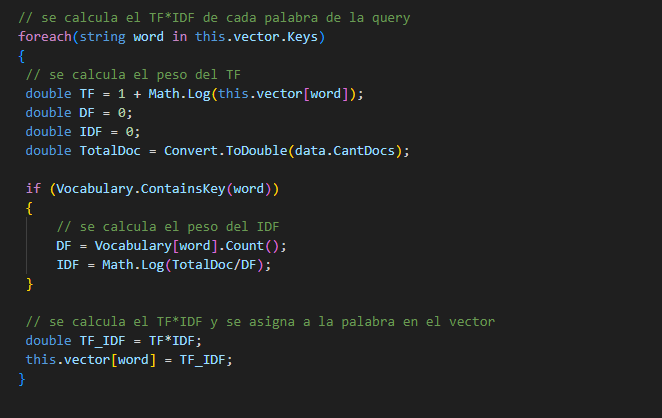
\includegraphics[width=12cm]{./img/tfidf.png}
        \end{figure}
        
        Como se puede apreciar, en el cálculo de los pesos \textbf{TF} e \textbf{IDF} no se utilizan los valores de frecuencia tal cual se encuentran, sino que se utilizan logaritmos. Esto se debe a que los valores sin transformar pueden generar una distorsión en los resultados.
        
        Por ejemplo, si utilizamos la frecuencia del término sin transformar, es posible que los términos más frecuentes (artículos, preposiciones, conjunciones) dominen la representación vectorial del documento, lo que puede resultar problemático ya que los términos más frecuentes no suelen ser los más importantes.  De manera similar, si utilizamos la frecuencia inversa del documento sin transformar, es posible que los términos raros sean demasiado ponderados, lo que puede ser problemático ya que los términos raros no siempre son los más relevantes.
        
        Resumiendo, el uso de logaritmos en el cálculo de \textbf{TF} e \textbf{IDF} ayuda a equilibrar la importancia de los términos en la representación vectorial de los documentos, y a mejorar la precisión de los resultados de la búsqueda.
        
        \subsubsection{Vectores de consulta y vectores del documento}
        Como la presencia de operadores determina características especiales para la búsqueda, no basta con crear en principio un vector de consulta, sino que se necesitará un vector para cada operador y un vector que contenga todos los términos de la consulta.
        
        Dichos vectores se estructuran como diccionarios \textbf{$<$string, double$>$}, donde las claves son los términos y los valores son su \textbf{TF*IDF} correspondiente. Tras una consulta, obtendremos:
        \begin{enumerate}
            \item Un vector \textbf{OR}, que contendrá todos los términos de la consulta, se encuentren o no marcados con un operador.
            \item Tantos vectores \textbf{NOT} como términos estén marcados con el operador “\textbf{!}”.
            \item Tantos vectores \textbf{MUST} como términos estén marcados con el operador “\textbf{\textasciicircum}”.
        \end{enumerate}
        Para crear los vectores de cada documento se procede de manera similar a la creación de los vectores de consulta. Se parte de ellos para determinar qué documentos contienen los términos de interés, y se asocia a cada término su \textbf{TF} en el documento. Nótese que no es necesario calcular el \textbf{IDF} del término, pues este valor solo determina su rareza en el cuerpo de documentos.
    \subsection{Cálculo de resultados}
    Construidos todos los vectores, solo resta determinar qué documentos serán devueltos y cuál será su orden. Para determinar la relevancia de un documento se le asignará una puntuación o \textbf{score}. El cálculo de dicho score se realiza con la segunda noción del modelo vectorial: la \textbf{similitud del coseno}.
       
    \subsubsection{Similitud del coseno}
        La \textbf{similitud del coseno} es una técnica de la recuperación de información que se utiliza para medir la similitud semántica entre dos vectores. Se calcula como el coseno del ángulo entre  dos vectores (en este caso, un vector de consulta y su correspondiente vector de documento), y se utiliza para medir cuán similares son una consulta y un documento. Un valor de similitud del coseno de 1 indica que los dos vectores son idénticos, mientras que un valor de 0 indica que los vectores son completamente diferentes.
        
        \begin{figure}[h]
                \centering
                \caption{Fórmula de similitud del coseno}
                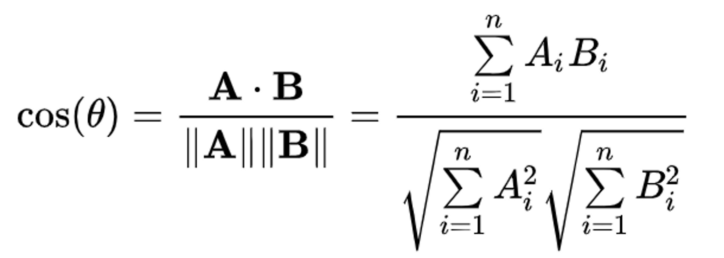
\includegraphics[width=10cm,height=3cm]{./img/simcos.png}
        \end{figure}    
       
        \newpage
        La similitud del coseno de los vectores de consulta se puede calcular como el producto escalar de ambos vectores normalizados. La normalización de un vector se realiza calculando en primer lugar la norma del vector, y luego dividiendo cada componente entre ella. En la fórmula anterior, se representan en el denominador las normas de los vectores A y B. En mi \textbf{Moogle!} se normalizan los vectores con el método \textbf{NormalizeVector} y se calcula su producto escalar con el método \textbf{GetAllScores}.
        
        \begin{figure}[h]
            \centering
            \caption{Método NormalizeVector}
            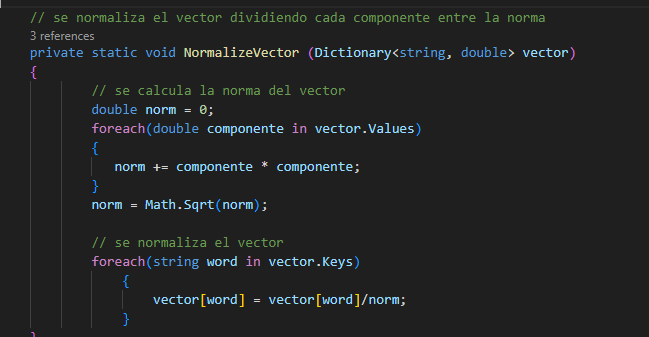
\includegraphics[width=12cm,height=6cm]{./img/normvec.png}
        \end{figure}
        
        \begin{figure}[h]
            \centering
            \caption{Método GetAllScores}
            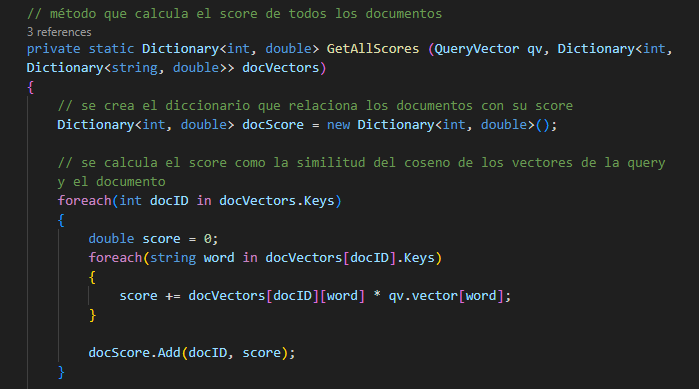
\includegraphics[width=12cm,height=6cm]{./img/getscore.png}
        \end{figure}
       
        \newpage
        \subsubsection{Normalización y producto escalar de los vectores}
        Todos los vectores de consulta y de documento se crean en el programa ya normalizados. Para devolver resultados lo más precisos posible, es necesario multiplicar un solo vector de consulta con un solo vector de documento. ¿Cómo se estructuran dichos vectores?
       
        Recordemos que teníamos varios vectores de consulta, y que a cada uno se le hacía corresponder un vector de documento. Para obtener el vector que devolverá los resultados más precisos, necesitamos operar el vector \textbf{OR} con los vectores \textbf{NOT} y \textbf{MUST} (cada vector NOT y MUST contiene un solo término).
        
        Comencemos por el caso más sencillo: los vectores \textbf{MUST}. Como toda palabra del vector \textbf{MUST} debe aparecer en los documentos que se devuelvan, se creará el diccionario de scores para los documentos que coincidan con el vector \textbf{OR} y aquellos que coincidan con los vectores \textbf{MUST}. Como las palabras de los vectores \textbf{MUST} deben necesariamente aparecer en todos los documentos encontrados, se eliminará del vector de resultados de \textbf{OR} todo documento que no coincida con el resultado de todos los vectores \textbf{MUST}. De esta forma queda conformada la colección de documentos que contienen las palabras que no pueden faltar en la respuesta.
       
        Para el caso de los vectores \textbf{NOT}, se eliminará del vector de resultados de \textbf{OR} todo documento que coincida con el resultado de alguno de los vectores \textbf{NOT}. De esta forma queda conformada la colección de documentos que no contienen las palabras que no pueden aparecer en la respuesta, quedando así conformada la colección que se devolverá como respuesta.

    \section{Devolución de los resultados}
    Los documentos que resultaron ser relevantes para el usuario según su consulta se devolverán ordenados según su \textbf{score}. En la interfaz de búsqueda, el usuario podrá conocer cuántos documentos coinciden con su búsqueda, cuáles son esos documentos en orden de relevancia y, por cada documento en la respuesta, recibirá la línea del texto que contenga la mayor cantidad de palabras relevantes en su búsqueda.

\end{document}